\documentclass[12pt,oneside]{report}
\usepackage[utf8]{inputenc}
\usepackage[T1]{fontenc}
\usepackage[english]{babel}
\usepackage{titlepic}
\usepackage{graphicx}
\usepackage[11pt]{moresize}
\usepackage{eso-pic}
\usepackage[export]{adjustbox}
\usepackage{fancyhdr}
\usepackage{vmargin}
\usepackage{titlesec}
\usepackage{textpos}
\usepackage{minted}
\usepackage{float}
\usepackage[breaklinks=true,hidelinks]{hyperref}
\usemintedstyle{manni}
\usepackage{xurl}
\usepackage{subfig}

\renewcommand{\thesection}{\arabic{section}}
\renewcommand{\thefigure}{\arabic{section}.\arabic{subsection}.\arabic{figure}}

\newcommand{\HRule}{\rule{\linewidth}{0.5mm}}

%%%% Footer and Header %%%%%%%%%%%%%%

\pagestyle{fancy}
\fancyhf{}
\fancyfoot[C]{\footnotesize{\rightmark}}
\fancyfoot[R]{Page -- \thepage}
\renewcommand{\footrulewidth}{0.5pt}
\renewcommand{\headrulewidth}{0pt}


% Redefine the plain page style
\fancypagestyle{plain}{
\fancyhf{}
\fancyfoot[C]{\footnotesize{\rightmark}}
\fancyfoot[R]{Page -- \thepage}
\renewcommand{\footrulewidth}{0.5pt}
\renewcommand{\headrulewidth}{0pt}
}

\begin{document}
%----------------------------------------------------------------------------------------
%	MARGINS
%----------------------------------------------------------------------------------------
\setmarginsrb{ 1.2in}   % left margin
             { 0.6in}   % top margin
             { 1.2in}   % right margin
             { 0.8in}   % bottom margin
             {  20pt}   % head height
             {0.25in}   % head sep
             { 9pt}     % foot height
             { 0.75in}  % foot sep

%%%%%%% Title Page %%%%%%%%%%%%%%%%%%%

%---title format---
%%%%%%%%%%%%%%%%%%%%%%%%%%%%%%%%%%%

\titleformat{\chapter}[display]
{\normalfont\Large\bfseries}
{} % label
{0.5ex} % sep
{
	\rule{\textwidth}{1pt}
	\vspace{1ex}
	\centering
} % before-code
[
\vspace{-0.5ex}%
\rule{\textwidth}{0.3pt}
] % after-code

\titlespacing*{\chapter} {0pt}{0mm}{2mm}   
%%%%%%%%%%%%%%%%%%%%%%%%%%%%%%%%%%%%

	\begin{titlepage}
		\begin{center}
			\vspace*{\fill}
			
 			\begin{figure}[h]
       	 		
\includegraphics[width=5cm, center]{Figures/Logo_ECAM.jpg}	
       	 	\end{figure}
 			\vspace{\baselineskip}
 			
       		\HUGE{Test Driven Development Project}
       		\vspace{0.5cm}


       		\normalsize{Décembre 2019} 
			
       		\vspace*{\fill}
       		
       		\large{DENIS Maxime 15089 \\\
                SMITS Victor 16107\\
                TOURNEUR Bernard 16148}
            \vspace{\baselineskip}
            
            \large{Ecole centrale des arts et métiers}
            \vspace{\baselineskip}
            
       		\small{MA1 -  Groupe 1}
       		\vspace{\baselineskip}
       		
       		\normalsize{Année académique 2019-2020}
   		\end{center}
	\end{titlepage}

%%%%% table of content %%%%%%
\tableofcontents

%%%%% Documents %%%%%%
\newpage
\section{Introduction}
    \paragraph{}
    Dans le cadre du cours \textit{Architecture logicielle}, il nous a été demandé, dans un premier temps d'établir un projet en \textit{Java}. L'important lors de la réalisation de ce projet était de mettre en place différents critères de qualité et de contrôler ceux-ci. Après 4 séances, les différents projets ont été redistribués à travers les groupes dans l'optique d'améliorer la qualité du programme et non sa fonctionnalité.

\paragraph{}
    Une fois le nouveau projet récupéré, il convient d'en faire une analyse approfondie ainsi qu'une analyse des différents critères de qualité mis en place. C'est sur base de ces critères que nous effectuerons notre travail de refactoring du code. Dans ce dossier se trouve les différentes analyses, problématiques, solutions et améliorations relatives à ce projet. Les objectifs atteints ou non y sont détaillés ainsi que les modifications apportées.

\paragraph{}
    L'ensemble du projet peut être trouver sur \textit{Github} \href{https://github.com/victorsmits/Ludotheque}{en cliquant ici} ou à l'adresse suivante: https://github.com/victorsmits/Ludotheque.

\paragraph{}
    L'intégration continue du projet a été réaliser grâce au système Jenkins et est retrouvable au \href{https://jenkins.ecam.be/login}{en cliquant ici} ou en vous rendant sur la platform jenkins de l'ecam dans le projet \textit{Ludotech}.
    \newpage
    
\section{Analyse de l'existant}
    \paragraph{}
Le projet du groupe 3\footnote{L'équipe composée de Louis Randriamora Andriantsiory, Kolawole Abdoulaye et Rudy Itunime Masala} consiste en la gestion d'une ludothèque, un centre de prêt de jeux en tout genre; jeux vidéos, jeux de société ou autres jouets.
\paragraph{}
Selon les spécificités décidées par le groupe 3, un jeu doit avoir un nom, un statut de disponibilité et un fabricant, quel que soit son type.\\
Certains types de jeux spécifiques ont des caractéristiques propres, ce qui entraîne l'utilisation de l'héritage, décrite au point \ref{subsection:structure}.
\paragraph{}
L'application devrait permettre au gérant de s'identifier, et de gérer la ludothèque; ajouter des jeux, faire des recherches, obtenir une liste de prêts, etc. \\
Elle devrait également permettre aux adhérents de faire des recherches de jeux, voyant lesquels sont disponibles ou non et de déclarer un emprunt.
\paragraph{}
L'application, codée en java, utilise les concepts de programmation orientée objet. La structure du programme est donc composée de classes représentant les différents objets ou acteurs intervenant. 

\subsection{Structure}
    \label{subsection:structure}
    \subsubsection{Classes et fonctionnalités}
        \begin{figure*}[h!]
                \centering
                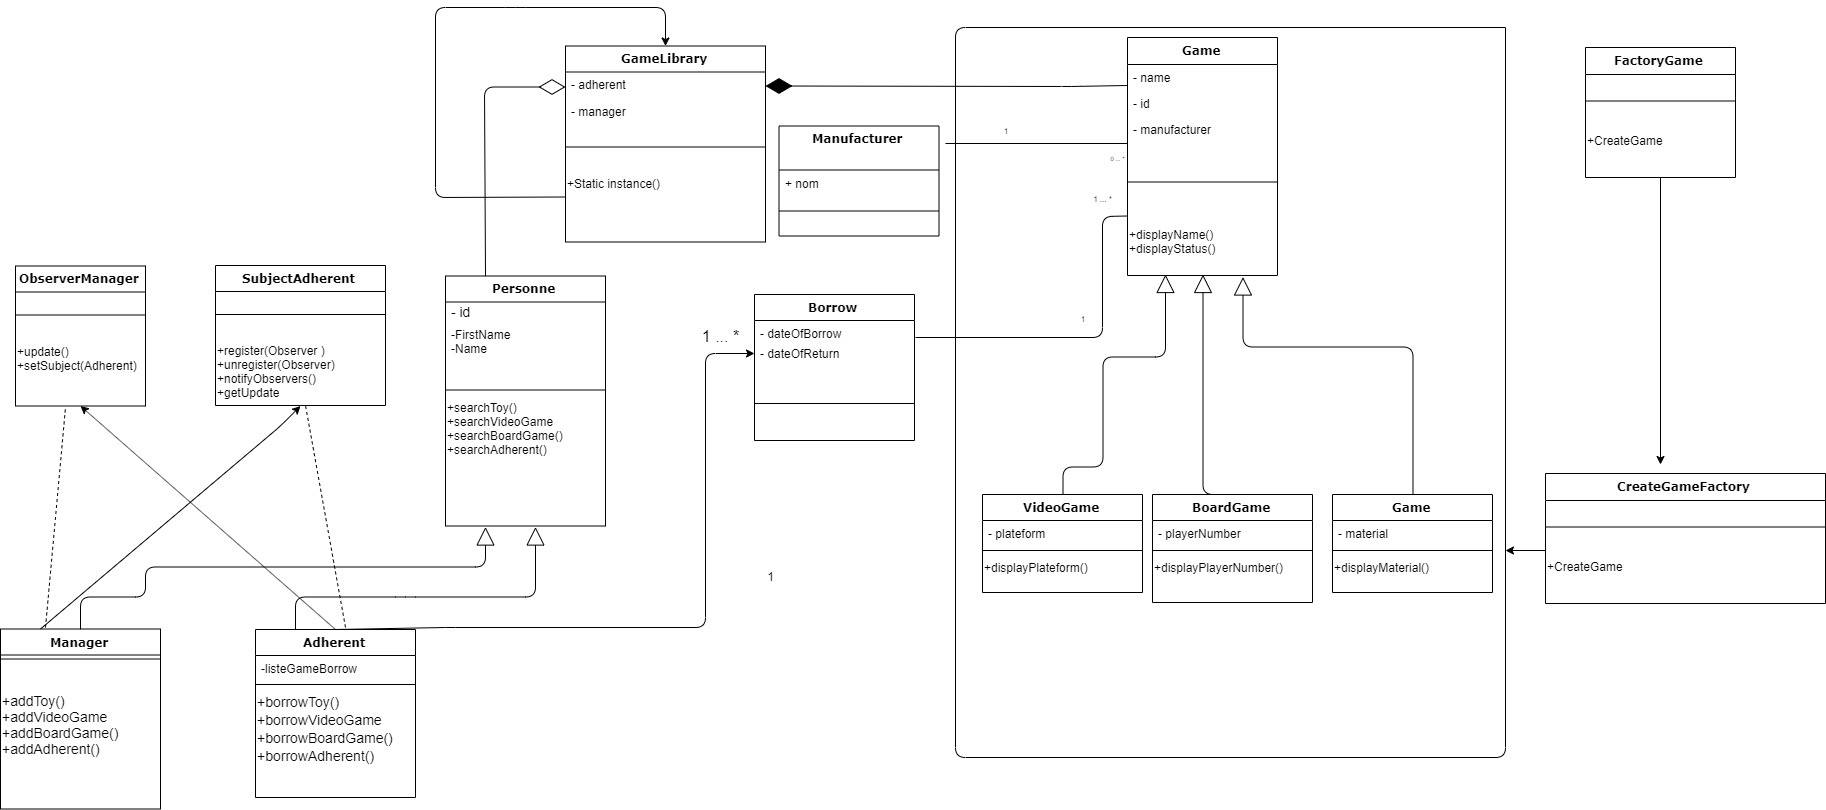
\includegraphics[width=\textwidth,center]{Figures/Class_Diagram.jpg}
                \caption{Diagramme de classe}
                \label{fig:classDiagram_old}
            \end{figure*}
        \newpage
        Le diagramme de classe en figure \ref{fig:classDiagram_old} représente la structure du projet que nous avons auditionné, et est repris en annexe en figure \ref{fig:annexe:classDiagram_old} pour plus de lisibilité.  
        \paragraph{}
        On observe sur ce diagramme que la première équipe de dévelopement avait créé une classe Game, de laquelle héritaient 3 sous-classes Game, BoardGame et VideoGame. Le diagramme ne semble pas à jour\footnote{Par rapport à l'état dans lequel nous avons récupéré le projet}, puisque la classe-fille Game a été remplacée par une classe Toy. 
        La super-classe Game est une classe abstraite et ne peut pas être implémentée.
        \paragraph{}
        4 différentes interfaces étaient présentes dans le code et ne sont pas reprises dans le diagramme de classe\footnote{AdherentFacade, ObserverManager, SubjectAdherent et UserFacade}. Ces interfaces sont des parties de design patterns qui seront décrits en sous-section \ref{subsubsection:design} : Design.
        \paragraph{}
        En outre, les relations entre les classes ne sont pas toutes claires, comme celle entre la classe Borrow et la classe Game, et celle entre la classe Manufacturer et la classe Game. Les aggrégations et compositions sont quant à elles plus claires; une GameLibrary est composée de Game, et a des Personne\footnote{Noté en français dans le diagramme de classe}, soit Manager soit Adherent.  
    \subsubsection{Design patterns}
        \label{subsubsection:design}
        \paragraph{}
        Le groupe 3 a choisi d'utiliser plusieurs designs patterns : l'observer, le facade, et le factory. \\
        Le design pattern observateur est utilisé pour envoyer des signaux à des modules, les observateurs. En cas de notification, les observateurs peuvent effectuer l'action adéquate en fonction des informations reçues. En pratique, le groupe 3 a implémenté l'observateur mais ne l'utilise pas. \\
        En effet, les interfaces ObserverManager et SubjectAdherent existent et présentent des méthodes typiques du design pattern (notifyObserver chez le subjectAdherent, setSubject qui est l'action de l'observateur), mais ne sont jamais utilisées et leurs méthodes jamais appelées. \\
        Le design pattern observer suit typiquement la structure représentée en figure \ref{fig:observer}.
        \begin{figure*}[h!]
                \centering
                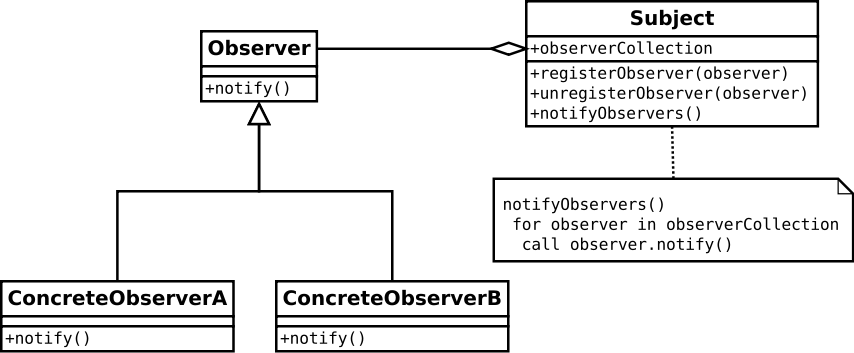
\includegraphics[width=\textwidth,center]{Figures/Observer.png}
                \caption{Design pattern observer}
                \label{fig:observer}
        \end{figure*}
        \newpage{}
        \paragraph{}
        Le design pattern factory permet d'instancier des objets héritant d'une classe abstraite, et donc d'instancier des objets dont la classe exacte est inconnue. \\
        Le factory est ici utilisé pour instancier des jeux, quel que soit leur types. Cependant, l'implémentation de ce design pattern n'était pas terminée et nous avons dû y apporter de nombreuses modifications. 
        \paragraph{}
        Le design pattern facade doit cacher une interface et conception complexe, en proposant au développeur ou utilisateur une interface plus simple et générique.\\
        Le UserFacadeImpl, qui implémentait une interface UserFacade\footnote{L'interface oblige le développeur à implémenter une méthode managerMenu, et une méthode adherentMenu, méthodes dont le rôle est de gérer un menu utilisateur}. A nouveau, de nombreuses modifications ont été apportées à la classe UserFacadeImpl.
        
    \subsubsection{Paradigmes}
        Le projet de ludothèque répondant à un problème concret, représentant une situation du monde réel, et comprenant des représentations d'objets physiques, la programmation orientée objet semble tout indiquée. \\ 
        Il existe une multitude de langages de programmation orientée objet; l'utilisation de Java est pertinente puisque c'est un langage de POO pour lequel de nombreux outils de qualités et d'intégration existent\footnote{C'est bien sûr le cas d'autres langages, mais la programmation Java faisait partie des exigences du client, le professeur}. 
        \paragraph{}
        Justifions la structure du projet et son design en fonction du problème auquel il répond.
        \newpage
        Le design pattern observateur semble servir à notifier le manager lorsqu'un adhérent s'enregistre, requièrant une action de ce dernier, probablement mettre à jour la base de données avec les informations de l'adhérent. Il est malheureusement difficile d'en être certain puisque le design pattern n'était pas utilisé dans le projet. 
        \paragraph{}
        La classe GameFactory permet de créer une instance de jeu, quel que soit son sous-type. La méthode principale (et unique) de cette classe est createGame, qui reçoit en paramètre les informations nécessaires à l'instanciation du jeu. Cette méthode ne respecte pas l'extensibilité, puisque si un développeur souhaite ajouter un autre type de jeu, il devra obligatoirement modifier la méthode createGame également. 
        \paragraph{}
        Le rôle de la classe UserFacadeImpl est de gérer l'interface utilisateur du programme. Puisque ce programme est exclusivement exécuté en terminal, sans interface graphique, cette classe appelle principalement des fonctions et classes terminales telles que println ou Scanner, qui alourdissent la lecture du code; il est donc intéressant de les placer dans une classe à part et non directement dans le main, ou dans une autre classe. 
        
\subsection{Critères de qualité}
    \paragraph{}
    La première équipe de développement a déclaré vouloir respecter les critères de qualité suivants : le projet doit être maintenable, respecter le concept d'intégrité, être "simple" et être extensible.\\ Le critère de simplicité est décrit par le groupe\footnote{Voir page 3 du rapport préliminaire du groupe} comme la facilité à comprendre la structure du projet et la logique des algorithmes et du code. 
    \paragraph{}
    La maintenabilité d'un logiciel décrit l'effort nécessaire pour comprendre, corriger ou modifier ce logiciel pour un développeur, extérieur au projet ou non. \\
    Le rapport préliminaire du groupe 3 indique qu'ils respectent ce critère par l'utilisation de la programmation orientée objet; il s'agit d'une erreur, puisque l'utilisation de la POO n'est pas garante de maintenabilité en soit.
    \paragraph{}
    Le critère de simplicité découle en réalité de celui de maintenabilité, et n'est donc pas un critère de qualité à part entière.  
    \paragraph{}
    L'intégrité, que le groupe déclare respecter à l'aide de tests unitaires, est la nécessité de conserver à tout moment une cohérence, pertinence et un fonctionnement correct du programme et des données exploitées.\\
    Les tests unitaires, s'ils sont eux mêmes intègres et  fonctionnels, peuvent valider que le programme a le fonctionnement attendu et que les données générées ou  traitées seront intègres. Ils ne sont cependant pas une garantie absolue d'intégrité, un aspect imprévu et non testé du logiciel pourrait passer au travers de la vérification par test.  
    \paragraph{}
    L'extensibilité est un sous-critère de la maintenabilité, et est la facilité avec laquelle un développeur peut ajouter des classes ou méthodes ou autres fonctionnalités au logiciel, en apportant un minimum d'autres modifications au code existant. Pour respecter ce critère, l'équipe avait choisi d'appliquer l'encapsulation, c'est-à-dire de masquer le fonctionnement interne des classes en proposant des interfaces; d'utiliser les relations d'héritage; et d'appliquer les designs patterns mentionnés précédemment. 

    \subsubsection{Métriques}
        \paragraph{}
        Lorsque notre équipe a récupéré le projet, aucun système de mesure de métrique n'était mis en place. 
        \paragraph{}
        Nous avons donc configuré un projet Jenkins permettant de relever certaines valeurs de qualité, notamment l'intégrité avec la réalisation automatique des tests unitaires; la qualité du style de codage (bien qu'elle ne se trouvait pas dans les critères du groupe 3) avec des tests automatiques détectant la duplication de code et appliquant le checkstyle Java de Google; nous avons utilisé le plugin CodeMR d'intellij, localement, pour réaliser une analyse des métriques de qualité du projet \footnote{Une liste des métriques mesurés par ce plugin peut être trouvée ici : \url{https://plugins.jetbrains.com/plugin/10811-codemr}}. 
        \paragraph{}
        Puisque de nombreux métriques sont utilisés par le plugin pour déterminer les différents niveaux de qualité (complexité, longueur, cohésion, couplage, etc), nous n'en expliquerons ici qu'une partie, concernant les critères choisis par le premier groupe.  
        \paragraph{}
        L'indice de McCabe est une valeur entière caractérisant la maintenabilité du code en déterminant , pour chaque méthode utilisée, la complexité de cette dernière. Ce calcul est fait en comptant le nombre de structures conditionnelles, de boucles et structures itératives, et de conditions bouléennes (\&\&, ||, etc). Plus l'index est grand, plus il sera difficile de coder un test unitaire couvrant correctement la méthode et plus cette méthode sera difficile à comprendre et/ou modifier. Une valeur acceptable serait de 4 ou 5\footnote{Source : \url{https://www.theserverside.com/feature/How-to-calculate-McCabe-cyclomatic-complexity-in-Java}}. Cet indice est utilisé dans le \textit{Weighted Method Count} du plugin, lui même utilisé pour déterminer la complexité des méthodes, donc des classes et donc du programme. Plus le programme est complexe, moins il sera maintenable.
        \paragraph{}
        Le couplage entre deux classes est l'intensité de la liaison entre ces classes, la dépendance qui existe entre ces classes. Ainsi, si une modification est appliquée à une des classes, il y aura des répercussions sur l'autre, ce qui peut entraîner une augmentation du temps de développement nécessaire. \\ 
        Le couplage est donc un indicateur de l'extensibilité du programme. Dans le plugin, il est défini par plusieurs métriques, notamment le \textit{Number of Children} qui indique le nombre de sous-classes directes d'une classe; le \textit{Coupling Between Object Classes} qui compte le nombre de classes à laquelle une certaine classe est couplée, en comptant le nombre de classes qui utilisent ses attributs ou méthodes; et le \textit{Access to Foreign Data} qui indique le nombre de classes dont les attributs sont atteignables par la classe en question. 
        
        \paragraph{}
        Puisque lorsque nous avons récupéré le projet, ce dernier n'était pas terminé et ne compilait pas, nous n'avons pas pu examiner l'intégrité du projet à l'aide de Jenkins; certains tests unitaires échouaient, et le projet Jenkins ne compilait pas initialement. Nous avons cependant rapidement découvert de nombreuses erreurs de styles qui seront décrites en détail plus loin. Nous avons réalisé des analyses lors du développement et des modifications que nous avons apporté, ainsi qu'une analyse finale de la qualité selon les métriques sus-mentionnés qui sera décrite dans la section \ref{section:quality}, et comparée avec les résultats des mêmes métriques sur l'ancienne version du projet, en l'état auquel nous l'avons récupéré.
    \newpage

\newpage
\section{Objectifs non atteints}
    \subsection{Encapsulation}
    \paragraph{}
        Comme expliqué ci-dessus, le programme utilise la programmation orientée objet. Cependant la règle "\textit{Liskov substitution principle}" qui permet de regrouper différents objets sous un même type et ainsi pouvoir éviter la duplication de code et assurer l'extensibilité du programme n'est pas respectée.
        
    \paragraph{}
        Les interfaces sont existantes mais ne sont pas utilisées correctement. Par exemple, les 3 types de jeux sont tous regroupés dans un type global, \textit{l'interface "Game"}. Mais un client a pour attributs 3 listes de jeux contenant chacune un type de jeux, au lieu de les regrouper dans une liste de \textit{Game}. 
        
        Cela a donc créé de nombreuses duplications de codes et erreurs d'exécution. L'encapsulation est donc présente mais pas utilisée correctement.
        
\vspace{\baselineskip}
\subsection{Intégrité}
    \paragraph{}
        L'intégrité du programme n'est pas atteinte. En effet lors de l'ajout d'un jeux dans le système, le programme lui octroie un id qui se veut unique. Cependant, l'id est généré sur base de la fonction "\textit{Math.random}" de la manière suivante: \textit{this.id =  (long) ((Math.random() * (9999 - 1000) + 1) + 1000);}. Ce qui peut techniquement ne pas donner des id uniques. En effet, il y a une probabilité non nulle que plusieurs id générés par le code soient identiques.
        
        Ceci peut entraîner des erreurs lors d'une recherche dans le système en fonction de l'id et ainsi donc affecter l'intégrité du système.
        
\vspace{\baselineskip}
\subsection{Simplicité}
    \paragraph{}
        Certaine partie du projet ne sont pas très compréhensible. Ces dernières nous ont rendus la tâche plus compliquée. Par exemple, l'utilisation du design pattern observer dans le projet. Son utilité n'est jamais expliquée et les classes observer sont intégrée au projet et implémentées mais jamais utilisées. 

\vspace{\baselineskip}
\subsection{Utilisation des façades}
    \paragraph{}
        Le projet utilise le design pattern façade pour créer l'interface dans le terminal. Cependant, dans certaines classes, par exemple dans la classe \textit{Manager}, nous pouvons retrouver la présence d'interface utilisateur. Ceci va à l'encontre du design pattern.

\vspace{\baselineskip}       
\subsection{Maintenabilité}
    \paragraph{}
        Le projet contient de nombreuses duplications de code, ce qui va à l'encontre de la maintenabilité du programme. Certaines de ces duplications n'étaient pas correctes et ont du être corriger pour pouvoir être refactorisées par la suite.
        
\vspace{\baselineskip}
\subsection{L'extensibilité}
    \paragraph{}
        L'utilisation des designs patterns Factory et Façades ainsi que de la programmation orienté objet permette de favoriser l'extensibilité du projet tout en ne devant pas intervenir dans l'interface utilisateur via l'utilisation de façade ou dans la création de jeux via GameFactory.
        
    \paragraph{}
        La classe GameFactory permet de créer une instance de jeu, quel que soit son sous-type. La méthode principale (et unique) de cette classe est createGame, qui reçoiten paramètre les informations nécessaires à l’instanciation du jeu. Cette méthodene respecte pas l’extensibilité, puisque si un développeur souhaite ajouter un autretype de jeu, il devra obligatoirement modifier la méthode createGame également.
        
    \paragraph{}
        En conclusion on peut dire que l'extensibilité est atteints et respecter dans certain cas mais que d'autre ne le sont pas du tout.
    \newpage
    
\newpage
\section{Objectifs atteints}
    \subsection{Simplicité}
    \paragraph{}
        L'utilisation du design pattern singleton est un choix intelligent en ce qui concerne les performances du programme.
        En effet l'utilisation d'un singleton améliore l'occupation en mémoire et la vitesse d'exécution en ne générant qu'une seul instance de l'objet \textit{Manager}.
        
\vspace{\baselineskip}       
\subsection{Test unitaire}
    \paragraph{}
        L'intégrité de l'entièreté du projet est assurée par les tests unitaires. Ils nous permettent de vérifier que chaque modifications ou améliorations apportées n'amène pas le programme à un dysfonctionnement.

\vspace{\baselineskip}       
\subsection{Rôle des utilisateurs}
    \paragraph{}
        Chaque utilisateur a des droits précis quant aux actions qu'il peut réaliser dans le programme. La distinction entre un client et un manager est assurée par la présence de 2 classe ( \textit{Adherent , Manager} ) ayant chacune des actions différentes sur le programme. Toutefois, certaines actions restent communes aux deux types d'utilisateurs. Pour rendre cela possible, l'équipe a appliqué l'héritage sur ces 2 classes en créant une classe commune, la classe \textit{Person}. Ainsi nous pouvons partager certaines méthodes entre le manger et l'adhérent tout en évitant la duplication de code.
    \newpage

\newpage
\section{Modifications apportées}
        \paragraph{}
    Une fois l'analyse du projet et des objectifs terminée, nous avons commencé le \textit{refactoring} du code.
    
\subsection{Anglais et commentaires}
    \paragraph{}
    Pour commencer nous avons, tout en parcourant le code, corrigé les erreurs d'anglais telles que "\textit{with success}" à la place de "\textit{with successfull}" ou "\textit{first name}" pour "\textit{firstname}". Dans un premier temps nous nous sommes arrêtés aux commentaires et noms de variables globales et locales afin de ne pas créer d'erreurs par la modification d'une méthode.
    \paragraph{}
    Toujours en parcourant le code, nous avons jugé la pertinence des différents commentaires. Dès lors nous avons supprimé ceux qui semblaient inutiles. En effet, \textit{un bon code ne nécessite pas de commentaire}, il est donc inutile de placer un commentaire comme en figure \ref{fig:uselessComment}. 
    
    \paragraph{}
    De plus, tout au long du code on retrouve des commentaires copiés-collés. Ceux-ci ne sont donc pas pertinents comme on peut le voir sur la figure \ref{fig:CopyPasteComment}. Le second commentaire "\textit{// Enter username and press Enter}" vient du fait qu'il y a une duplication de code, ou au moins deux codes très similaires, probablement qu'un copié-collé a été fait sans modifier le commentaire. D'autre part, comme dis dans le paragraphe précédent, un commentaire de ce type n'est pas nécessaire à cet endroit. Une équipe de développement pourrait aisément comprendre ces quelques lignes de code.
    
\subsection{Noms des méthodes, classes et variables}
    
    \paragraph{}
    Comme précisé ci-dessus, la première équipe de développement a mis en place certaines conventions par rapport aux noms des classes et des variables. Pour vérifier ces conventions nous avons appliqué la même méthode qu'au point précédent, c'est à dire que tout en parcourant le code nous avons corrigé les différentes erreurs remarquées. Contrairement au point précédent, ces conventions étaient généralement respectées. Il a toutefois fallu corriger certains noms de variables, méthodes et classes, par exemple en figure \ref{fig:CodeBorrowGame} à la ligne 2 pour "\textit{boardGame}". Pour finir, il n'y avait rien de préciser quant aux méthodes, nous avons donc appliqués la même règle que pour les classes.
    
\subsection{Duplication de code}

    \paragraph{}
    A de nombreuses reprises nous avons observé des duplications de code. Ceux-ci sont dûs au fait que les relations d'héritage n'ont pas été utilisées comme elles l'auraient dû. Comme on peut le voir dans les figures \ref{fig:CodeBorrowGame} et \ref{fig:CodeborrowToy}, ces deux méthodes sont quasiment identiques. Les seules choses qui peuvent différencier ces deux méthodes sont la variable "\textit{boardGame}" ou "\textit{Toy}" et les chaînes de caractères dans les "\textit{switch}". Dans le code d'origine il existait une troisième méthode, identique aux deux premières mais pour "\textit{VideoGame}".
    
    \paragraph{}
    Pour palier à ce problème, nous avons réécrit une nouvelle méthode qui remplace les trois précédentes. Pour ce faire, nous avons utilisé les relations d'héritage entre "\textit{Game}" et "\textit{boardGame}", "\textit{toy}" et "\textit{VideoGame}". Cette méthode prend en paramètre le type du jeu en \textit{string}, une liste de \textit{Game} qui correspond à la base de données et un id de type \textit{long} caractérisant le jeu emprunté. Cela nous permet de faire une méthode générale qui sera valable pour les trois types de \textit{Game}. Elle renvoie un string qui nous informe sur le résultat de la tentative d'emprunt. Cette méthode peut être observée en figure \ref{fig:Codeborrow}.
    
\subsection{Erreurs de \textit{checkstyle}}

    \paragraph{}
    Lorsque nous avons pris en main le projet nous avions un nombre élevé d'erreurs de \textit{checkstyle}. La plupart étaient des erreurs de longueur de ligne ou de d'espacement entre les différentes boucles, méthodes, variables et classes. Pour corriger celles-ci nous avons utilisé \textit{Jenkins} qui permet de repérer ces différentes erreurs sur base d'un template. Une fois les erreurs définies, il a suffit d'appliquer les bonnes règles aux différents endroit renseignés sur \textit{Jenkins.}
    \newpage
    
\section{Qualité du projet}
    \label{section:quality}
L'intégration avec Jenkins nous a permis de valider l'intégrité du projet au fur et à mesure que nous développions. Les tests unitaires étaient en effet effectués automatiquement.......... \\
Pour réaliser la mesure de métriques de qualité du projet, nous avons utilisé un plugin d'intellij nommé CodeMR, qui génère automatiquement un rapport contenant les résultats d'un grand nombre de métriques de qualité selon plusieurs critères. 
\\ Les fichiers html générés sont placés automatiquement dans le sous-dossier \path{/codemr/Ludotheque/html}
\footnote{Rapport qualité : \url{https://github.com/victorsmits/Ludotheque/tree/master/codemr/Ludotheque/html/main_report}}.

\subsection{Taille}
    \begin{figure}[h!]
        \centering
        \subfloat[Ancienne taille.]{{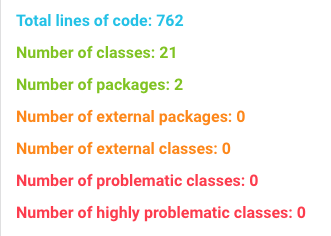
\includegraphics[width=0.45\textwidth]{Figures/Old_Size.png}}}
        \qquad
        \subfloat[Nouvelle taille.]{{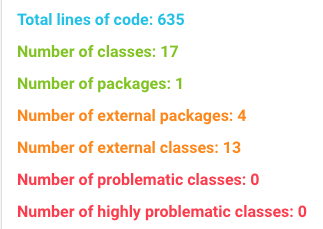
\includegraphics[width=0.45\textwidth]{Figures/New_Size.png}}}
        \caption{Taille du projet.}
    \end{figure}
La taille du code a diminué de manière non négligeable; diminution de 16\% du nombre de lignes de code, expliquée principalement par la suppression de nombreuses duplications de code ; et diminution de 19\% du nombre de classes dans le projet, expliqué par la suppression de plusieurs classes entièrement redondantes et non implémentées. 
\paragraph{}
La diminution de la taille du code pour une même qualité globale entraîne souvent une meilleure lisibilité du code, et donc une augmentation de sa maintenabilité. 
\newpage
\subsection{Complexité}

    \begin{figure}[h!]
        \centering
        \subfloat[Ancienne Complexité interne.]{{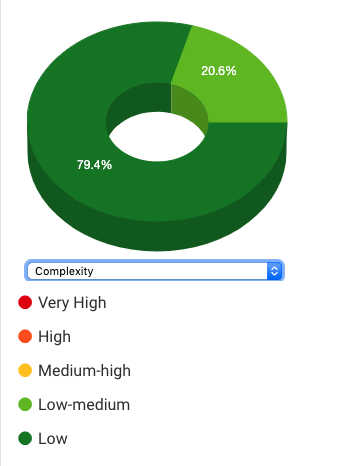
\includegraphics[width=0.47\textwidth]{Figures/Old_Complex.png}}}
        \qquad
        \subfloat[Nouvelle complexité interne.]{{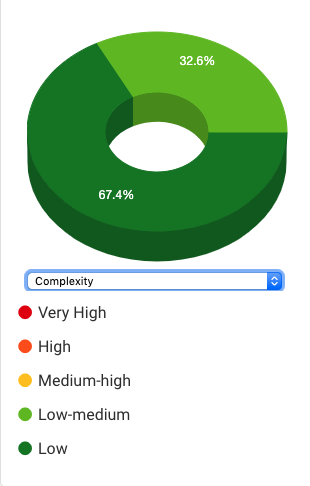
\includegraphics[width=0.4\textwidth]{Figures/New_Complex.png}}}
        \caption{Complexité générale.}
    \end{figure}
On constate que la complexité du projet a augmenté avec nos modifications, donc que la qualité du projet a décru en ce qui concerne la maintenabilité; ceci est probablement expliqué par le fait que nous avons implémenté plusieurs classes et méthodes qui étaient laissées vides par l'équipe précédente, nous avons notamment fait augmenter les indices de McCabe, les interactions entre les classes, etc. Les valeurs de métriques de complexité du projet tel que nous l'avons reçu ne sont donc pas représentatives de la complexité réelle du design initial. 

\newpage
\subsection{Cohésion}
    \begin{figure}[h!]
        \centering
        \subfloat[Ancien manque de cohésion interne.]{{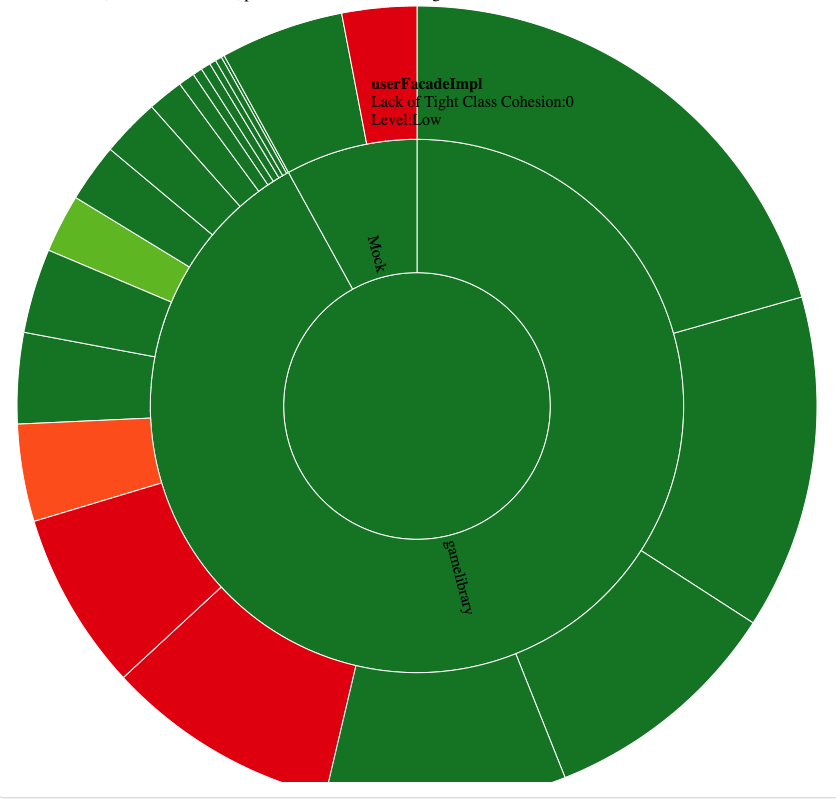
\includegraphics[width=0.45\textwidth]{Figures/Old_Cohesion.png}}}
        \qquad
        \subfloat[Nouveau manque de cohésion interne.]{{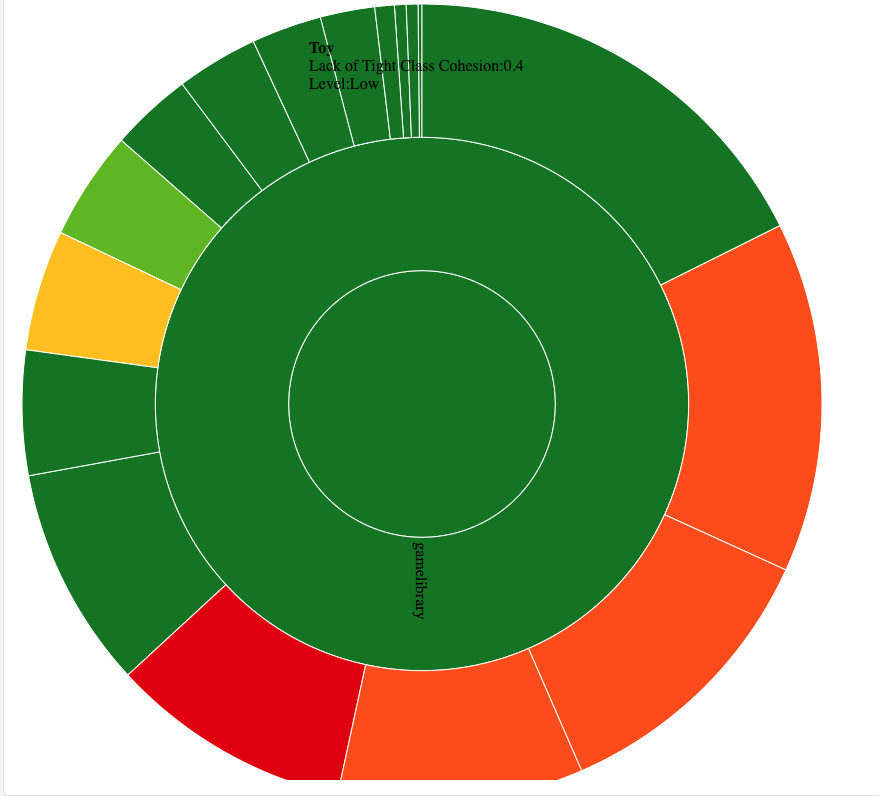
\includegraphics[width=0.45\textwidth]{Figures/New_Cohesion.png}}}
        \caption{Manque de cohésion. Chaque portion de disque représente une classe du projet; sa couleur, le taux de manque de cohésion.}
    \end{figure}
    \begin{figure}[h!]
        \centering
        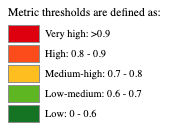
\includegraphics{Figures/Legend.png}
        \caption{Légende}
    \end{figure}
Ce paramètre décrit la qualité des relations à l'intérieur d'une classe (utilisation de tous les attributs par les méthodes de la classe donc pas d'attribut inutile, par exemple); une cohésion élevée (donc vert, manque de cohésion bas) est associé avec des qualités telles que la robustesse et la maintenabilité. En modifiant le code, nous avons globalement amélioré la cohésion du programme, même si certaines classes telles que Person ou Authentification se sont dégradées, ce qui s'explique par le fait que nous avons ajouté de nombreuses méthodes à cette classe.  

\newpage
\subsection{Couplage}
    \begin{figure}[h!]
        \centering
        \subfloat[Ancien couplage interne.]{{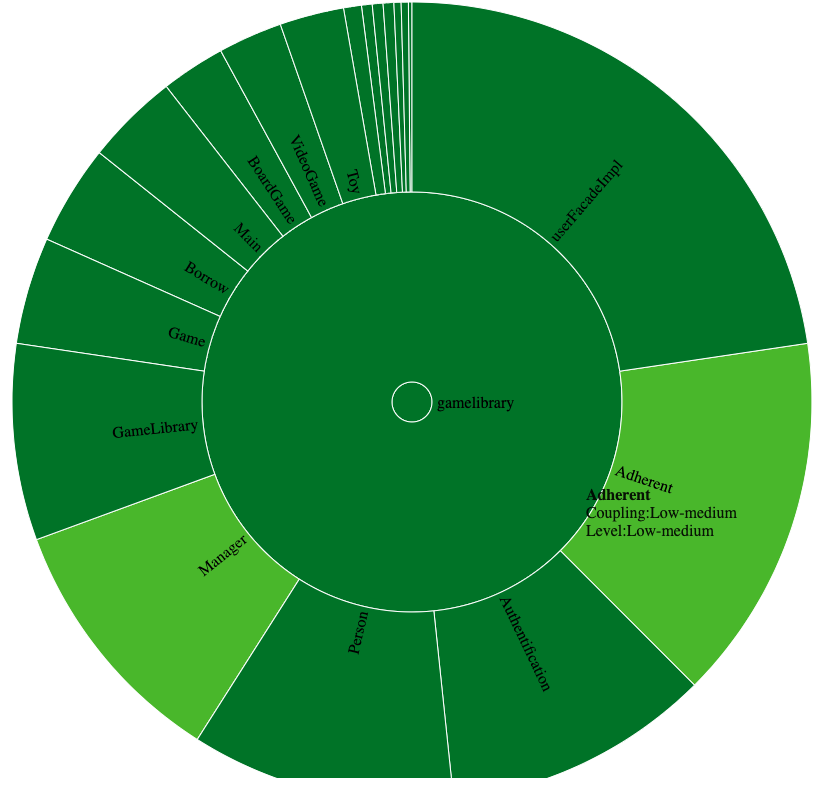
\includegraphics[width=0.45\textwidth]{Figures/Old_Coupling.png}}}
        \qquad
        \subfloat[Nouveau couplage interne.]{{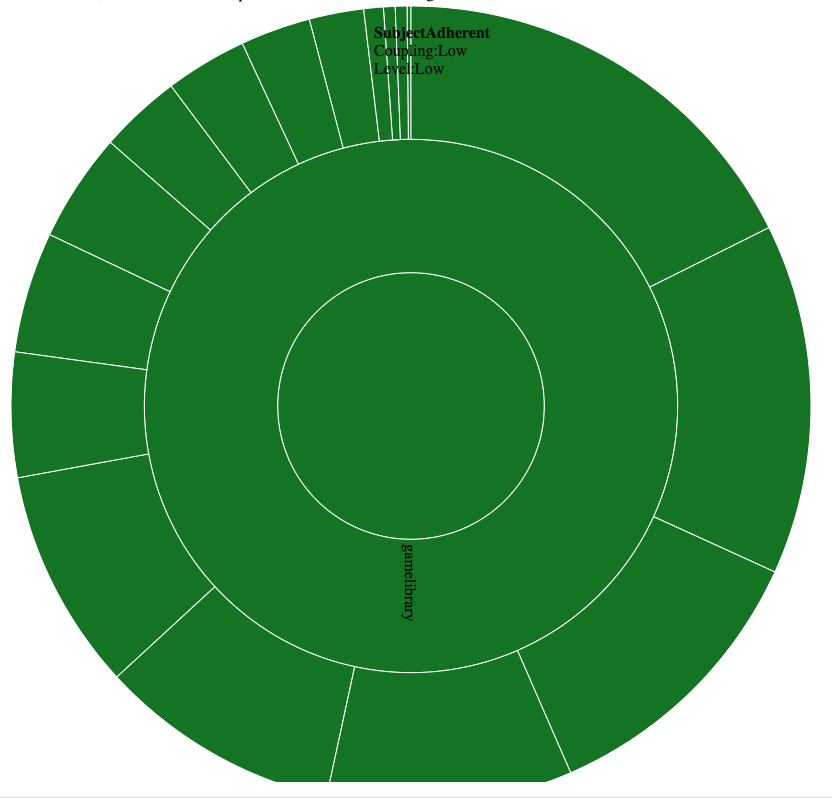
\includegraphics[width=0.45\textwidth]{Figures/New_Coupling.png}}}
        \caption{Couplage interne.}
        \label{fig:couplage_interne}
    \end{figure}
    \begin{figure}[h!]
        \centering
        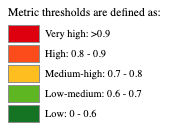
\includegraphics{Figures/Legend.png}
        \caption{Légende}
    \end{figure}
    \paragraph{}
    Nous pouvons constater que le couplage entre les classes a légèrement diminué \footnote{Le couplage des classes Adherent et Manager a diminué}. Cependant, puisque nous n'avons presque pas changé la structure du programme, il semble logique que le couplage entre les classes n'ait presque pas changé. Ce couplage relativement bas implique que le projet devrait être facilement extensible.

\newpage
\subsection{Erreur de Style}
    \begin{figure}[h!]
        \centering
        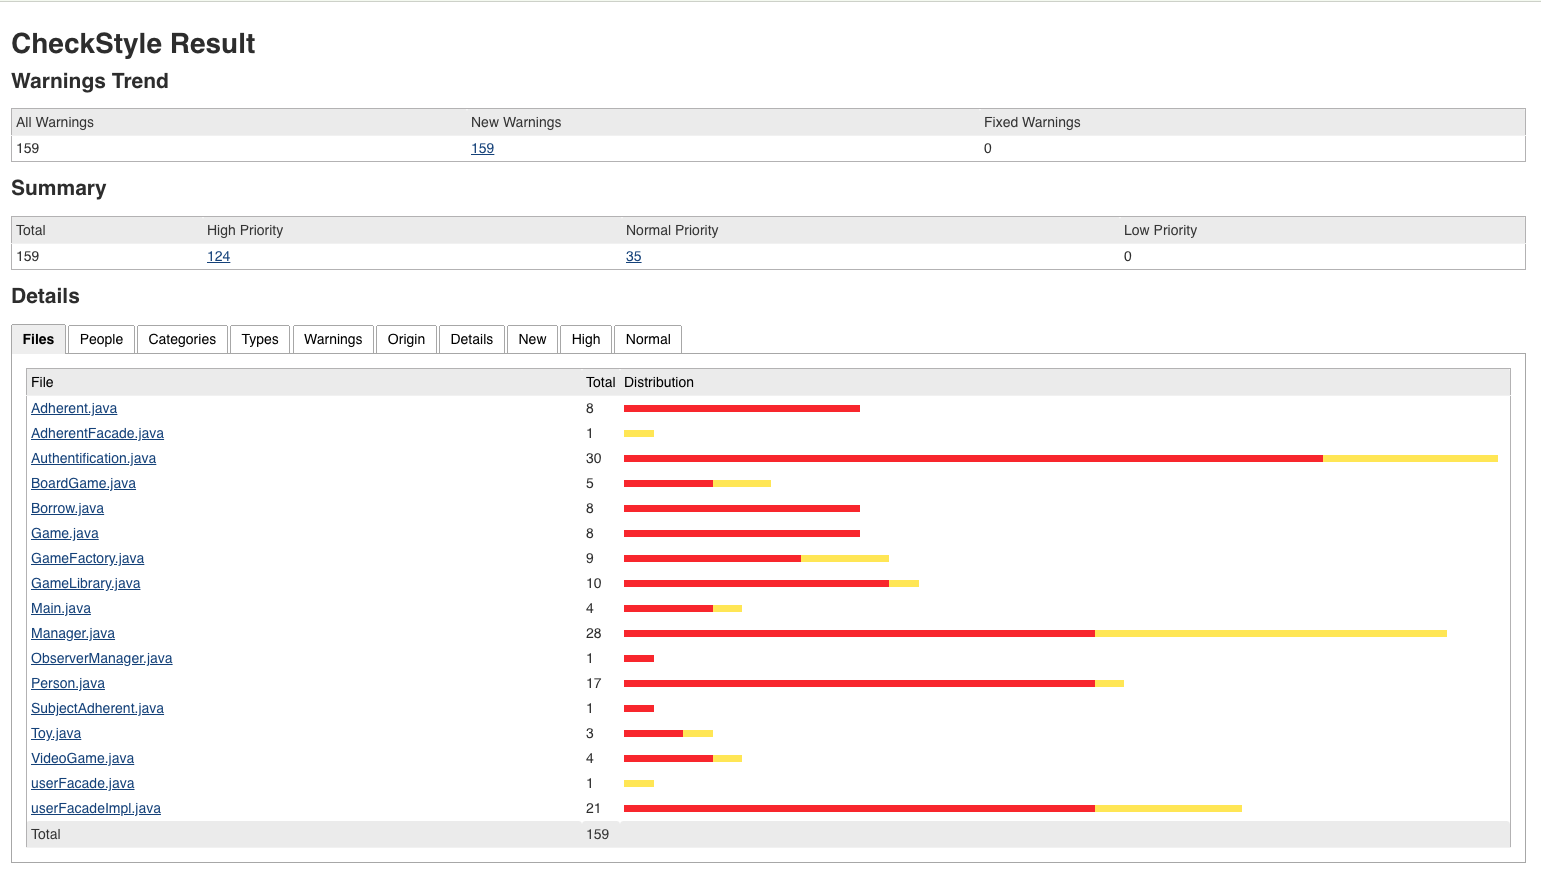
\includegraphics[width=0.8\textwidth]{Figures/Old_CheckStyle.png}
        \caption{Ancienne erreur de style.}
        \label{fig:checkstyle}
    \end{figure}
    
    \paragraph{}
    Comme nous pouvons le voire dans la figure \ref{fig:checkstyle} la première version du code contenait de nombreuse erreur de style de code.
    Nous avons donc résolut toutes les erreurs de check Style qui ont été repérée par Jenkins via la comparaison aux règles de codage de Google.
    \newpage
    
\section{Conclusion}
    \paragraph{}
Pour clôturer ce travail, il convient de rappeler que l'analyse du projet existant nous a permis de déterminer la qualité du code. Ceci grâce aux différents critères de qualité qui ont été mis en place et décidés par la première équipe de développement. Certains de ces critères étaient respectés et appliqués correctement dans le code. Le couplage entre classes est en effet assez faible, ce qui est un indicateur qu'il ne sera pas trop difficile d'apporter des modifications au projet; il est relativement extensible, malgré quelques défauts. 
\\
Toutefois une partie des critères n'ont pas été respectés ou pas entièrement. Il convenait donc de modifier le code pour en augmenter la qualité et respecter les critères mis en place. La complexité du projet est également relativement basse ou moyenne; cependant la cohésion est globalement assez mauvaise, ce qui indique que des améliorations peuvent être apportées au projet pour augmenter sa maintenabilité. 

\paragraph{}
Enfin, il convient de dire qu'il n'y pas de "recette" quant à la qualité d'une application. Les critères qui détermine cette qualité doivent être défini au préalable par l'équipe de développement selon les besoins de l'application. Il ne faut pas se fier à un seul critère de qualité ni se jeter sur ceux que l'on connaît. Il est donc important d'effectuer une analyse approfondie des besoins que l'application doit remplir afin d'en déterminer les critères de qualité adéquats.
    \newpage
    
\section{Glossaire}
    \begin{description}
    \item[S O L I D : ]Single responsibility principle, Open/closed principle, Liskov substitution principle, Interface segregation principle, Dependency inversion principle.
\end{description}
    \newpage
    
\section{Annexes}
    \subsection{Annexe 1 - Codes}

    \begin{figure*}[h!]
        \centering
        \begin{minted}[
frame=lines,
framesep=2mm,
baselinestretch=1.2,
fontsize=\footnotesize,
linenos
]
{csharp}

System.out.println("Enter your name"); //Enter name
\end{minted}
        \caption{Commentaire inutile}
        \label{fig:uselessComment}
    \end{figure*}
    
    \begin{figure*}[h!]
        \centering
        \begin{minted}[
frame=lines,
framesep=2mm,
baselinestretch=1.2,
fontsize=\footnotesize,
linenos
]
{csharp}

//put  username
Scanner user = new Scanner(System.in);
String username;
System.out.println("Enter your username"); // Enter username and press Enter
username = user.nextLine();

// put password
Scanner pass = new Scanner(System.in);
String password;
System.out.println("Enter your password");  // Enter username and press Enter
password = pass.nextLine();
\end{minted}
        \caption{Commentaires copiés-collés}
        \label{fig:CopyPasteComment}
    \end{figure*}
    
    \begin{figure*}[h!]
        \centering
        \begin{minted}[
frame=lines,
framesep=2mm,
baselinestretch=1.2,
fontsize=\footnotesize,
linenos
]
{csharp}

public String borrowBoardGame(long id){
    BoardGame boardgame;
    Borrow borrow;
    
    int count = 0;
    
    if(GameLibrary.getBoardGameList().isEmpty()){ // if database empty
        return "No board game in database";
    }
    
    for (int i = 0; i < GameLibrary.getBoardGameList().size(); i++) {
        if(GameLibrary.getBoardGameList().get(i).getId() == id ){ // if found
            
            if(GameLibrary.getBoardGameList().get(i).getStatut() == true){
                boardgame = GameLibrary.getBoardGameList().get(i);
                boardgame.setStatut(false);

                borrow = new Borrow(this, boardgame);

                GameLibrary.getAllBorrowList().add(borrow);
                borrowList.add(borrow);

                count = 1;
            }else{
                count = 2;
            }
            
        }
    }
    
    switch (count) {
        case 1:
            System.out.println("Please, go pick your borrow");
            return "Borrow with successfull";
        case 2:
            return "this game is not available";
        default:
            // if no found
            return "No found";
    }
    
}
\end{minted}
        \caption{Méthode "borrowBoardGame"}
        \label{fig:CodeBorrowGame}
    \end{figure*}
    
    \begin{figure*}[h!]
        \centering
        \begin{minted}[
frame=lines,
framesep=2mm,
baselinestretch=1.2,
fontsize=\footnotesize,
linenos
]
{csharp}

public String borrowToy(long id){
    Toy toy;
    Borrow borrow;
    
    int count = 0;
    
    if(GameLibrary.getToyList().isEmpty()){ // if database empty
        return "No toy in database";
    }
    
    for (int i = 0; i < GameLibrary.getToyList().size(); i++) {
        if(GameLibrary.getToyList().get(i).getId() == id ){ // if found
            
            if(GameLibrary.getToyList().get(i).getStatut() == true){
                toy = GameLibrary.getToyList().get(i);
                toy.setStatut(false);

                borrow = new Borrow(this, toy);

                GameLibrary.getAllBorrowList().add(borrow);
                borrowList.add(borrow);

                count = 1;
            }else{
                count = 2;
            }
            
        }
    }
    
    switch (count) {
        case 1:
            System.out.println("Please, go pick your borrow");
            return "Borrow with successfull";
        case 2:
            return "this toy is not available";
        default:
            // if no found
            return "No found";
    }
 
}
\end{minted}
        \caption{Méthode "borrowToy"}
        \label{fig:CodeborrowToy}
    \end{figure*}
    
    \begin{figure*}[h!]
        \centering
        \begin{minted}[
frame=lines,
framesep=2mm,
baselinestretch=1.2,
fontsize=\footnotesize,
linenos
]
{csharp}

private String borrowGame(String gameType,
                              ArrayList<Game> database,
                              long id) {
    Game game;
    Borrow borrow;
    int count = 0;

    if (GameLibrary.getVideoGameList().isEmpty()) {
        return "No video game in database";
    }

    for (Game value : database) {
        //Check if game exist
        if (value.getId() == id) {
            //Check the game status
            if (value.getStatus()) {
                game = value;
                game.setStatus(false);

                borrow = new Borrow(this, game);

                GameLibrary.getAllBorrowList().add(borrow);
                borrowList.add(borrow);

                count = 1;
                break;
            } else {
                count = 2;
            }

        }
    }
    switch (count) {
        case 1:
            return "You can pick up your " + gameType + ".";
        case 2:
            return "This " + gameType + " is not available.";
        default:
            return "This " + gameType + " was not found.";
    }
}
\end{minted}
        \caption{Méthode "borrowGame"}
        \label{fig:Codeborrow}
    \end{figure*}
    \newpage{}
    \label{annexe:classDiagram_old}
    \begin{figure*}[h!]
            \centering
            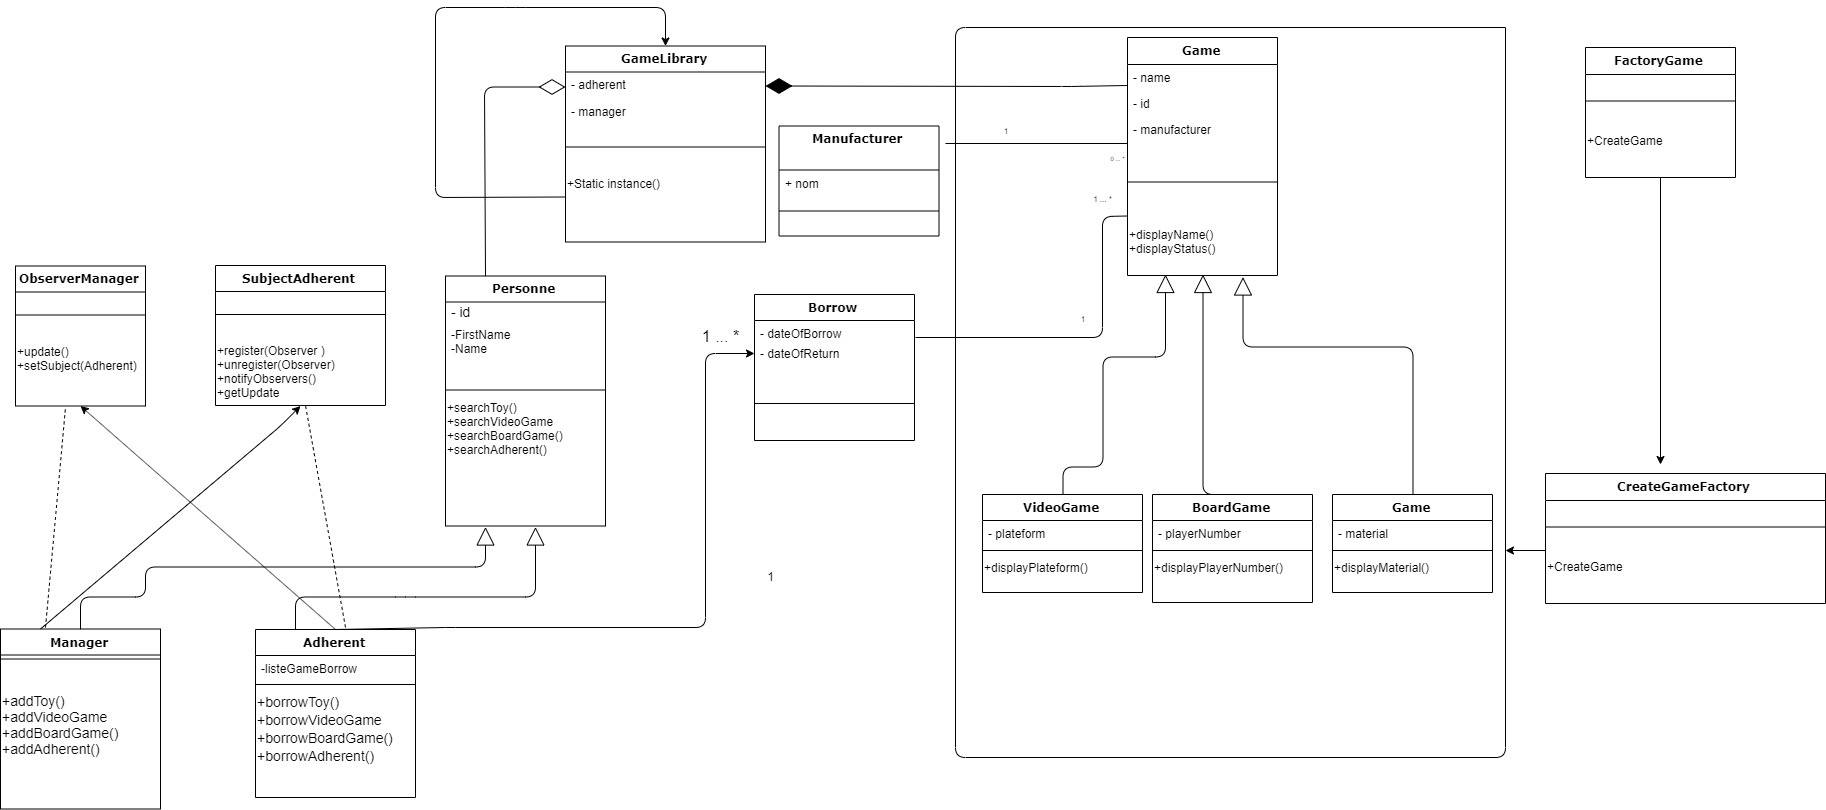
\includegraphics [scale=0.35, angle=90]{Figures/Class_Diagram.jpg}
            \caption{Diagramme de classe}
            \label{fig:annexe:classDiagram_old}
        \end{figure*}
    \newpage
    
\end{document}